\documentclass{beamer}

\usepackage{graphicx}
\usepackage{hyperref}
\usepackage[latin1]{inputenc}
\usepackage[T1]{fontenc}
\usepackage[english]{babel}
\usepackage{listings}
\usepackage{xcolor,mathrsfs,url}
\usepackage{amssymb}
\usepackage{amsmath}
\usepackage{ifthen}


% The command to define a subsection is '\subsec{}' and NOT '\subsection'.
% This code generates the bar. Don't edit.
\newcommand{\midbarnew}{}
\newcommand{\subsec}[1]
{
  \ifthenelse{\equal{#1}{}}
  {\renewcommand{\midbarnew}{} \subsection{}}
  {\renewcommand{\midbarnew}{ $\mid$ } \subsection{#1}}
}

% change the pictures here, if necessary. logobig and logosmall are the internal names
% for the pictures: do not modify them, just change "hulogo" and "logo". Pictures must be 
% supplied as JPEG, PNG or PDF
%########################################

\pgfdeclareimage[height=2cm]{logobig}{logo} % use hucase instead for the Humboldt-Case Logo
\pgfdeclareimage[height=1cm]{logosmall}{logo}

% use this number to modify the scaling of the headline on titlepage
\def\titlescale{1.0}


\title{Trade Policy: Part Two}
\author{Instructor: David Jinkins\thanks{I wish to acknowledge Battista Severgnini for providing last year's slides to me. His generosity saved me much time, and these slides are partially based on his. Any errors are of course my own.}}
\date{Date: Sept. 25, 2014}
%Start of the document
\begin{document}

\frame[plain]{% create the titleslide, layout controlled in metricsbeamer
	\titlepage
}

\frame{% how to print
\frametitle{Last time}
Chapter 8:
\begin{itemize}
\item Trade costs and Firm Behavior
\item Dumping
\item Multinationals
\end{itemize}
Chapter 9 : 
\begin{itemize}
\item Tariffs
\item Consumer \& Producer Surplus
\item Export Subsidies and other instruments
\end{itemize}
}

\frame{% how to print
\frametitle{Plan for Today}
\begin{itemize}
    \item Chapter 10 : Politics and Trade Policy
    \begin{itemize}
        \item Some additional arguments for Free Trade
        \item Arguments Against Free Trade
        \begin{itemize}
            \item National Welfare reasons 
            \item Income Distribution and Trade Policy
        \end{itemize}
        \item International Negotiations
        \begin{itemize}
            \item Some theory
            \item A short history of International Trade Agreements 
            \item Preferential Trade Arrangements
        \end{itemize}
    \end{itemize}
    \item Chapter 11 : Developing Countries and Trade Policy
    \begin{itemize}
        \item Rise and Fall of Import Substitution 
        \item Export Oriented Industrialization
    \end{itemize}
    \item Chapter 12: Trade Policy Controversy
    \begin{itemize}
        \item More Arguments for an Activist Trade Policy
        \item Trade \& the Environment
    \end{itemize}
\end{itemize}
}

\begin{frame}{But first a Review}

    \begin{itemize}
        \item Begin review
    \end{itemize}

\end{frame}

\frame[plain]{\includegraphics[page=37,width=\textwidth]{trade_policy_one.pdf}}
\frame[plain]{\includegraphics[page=39,width=\textwidth]{trade_policy_one.pdf}}
\frame[plain]{\includegraphics[page=41,width=\textwidth]{trade_policy_one.pdf}}
\frame[plain]{\includegraphics[page=32,width=\textwidth]{trade_policy_one.pdf}}
\frame[plain]{\includegraphics[page=43,width=\textwidth]{trade_policy_one.pdf}}
\frame[plain]{\includegraphics[page=44,width=\textwidth]{trade_policy_one.pdf}}
\frame[plain]{\includegraphics[page=48,width=\textwidth]{trade_policy_one.pdf}}
\frame[plain]{\includegraphics[page=56,width=\textwidth]{trade_policy_one.pdf}}
\frame[plain]{\includegraphics[page=57,width=\textwidth]{trade_policy_one.pdf}}
\frame[plain]{\includegraphics[page=58,width=\textwidth]{trade_policy_one.pdf}}
\frame[plain]{\includegraphics[page=59,width=\textwidth]{trade_policy_one.pdf}}
\frame[plain]{\includegraphics[page=60,width=\textwidth]{trade_policy_one.pdf}}
\frame[plain]{\includegraphics[page=61,width=\textwidth]{trade_policy_one.pdf}}
\frame[plain]{\includegraphics[page=62,width=\textwidth]{trade_policy_one.pdf}}
\frame[plain]{\includegraphics[page=63,width=\textwidth]{trade_policy_one.pdf}}
\frame[plain]{\includegraphics[page=64,width=\textwidth]{trade_policy_one.pdf}}
\frame[plain]{\includegraphics[page=65,width=\textwidth]{trade_policy_one.pdf}}
\frame[plain]{\includegraphics[page=66,width=\textwidth]{trade_policy_one.pdf}}
\frame[plain]{\includegraphics[page=69,width=\textwidth]{trade_policy_one.pdf}}
\frame[plain]{\includegraphics[page=70,width=\textwidth]{trade_policy_one.pdf}}
\frame[plain]{\includegraphics[page=72,width=\textwidth]{trade_policy_one.pdf}}
\frame[plain]{\includegraphics[page=75,width=\textwidth]{trade_policy_one.pdf}}
\frame[plain]{\includegraphics[page=76,width=\textwidth]{trade_policy_one.pdf}}
\frame[plain]{\includegraphics[page=77,width=\textwidth]{trade_policy_one.pdf}}
\frame[plain]{\includegraphics[page=80,width=\textwidth]{trade_policy_one.pdf}}
\frame[plain]{\includegraphics[page=81,width=\textwidth]{trade_policy_one.pdf}}
\frame[plain]{\includegraphics[page=83,width=\textwidth]{trade_policy_one.pdf}}
\frame[plain]{\includegraphics[page=86,width=\textwidth]{trade_policy_one.pdf}}
\frame[plain]{\includegraphics[page=88,width=\textwidth]{trade_policy_one.pdf}}

\begin{frame}

    \begin{itemize}
        \item End review!
    \end{itemize}

\end{frame}

\begin{frame}{Chapter 10 : Politics and Trade Policy}

    \begin{itemize}
        \item Some additional arguments for Free Trade
        \item Arguments Against Free Trade
        \begin{itemize}
            \item National Welfare reasons 
            \item Income Distribution and Trade Policy
        \end{itemize}
        \item International Negotiations
        \begin{itemize}
            \item Some theory
            \item A short history of International Trade Agreements 
            \item Preferential Trade Arrangements
        \end{itemize}
    \end{itemize}

\end{frame}

\begin{frame}{Some more arguments for Free Trade}

\begin{itemize}
    \item Chap. 1-8: gains from trade
    \item What else?
    \begin{itemize}
        \item Stuff we sort of already talked about
        \item The rent seeking distortions
        \item Politics and corruption
    \end{itemize}
\end{itemize}

\end{frame}

\begin{frame}{Stuff we already mentioned}

    \begin{itemize}
        \item Efficiency losses for small countries making tariffs
        \item Economies of scale, trade barriers reduce market size 
        \item Innovation, hard to pick winners
        \item Gains from shifting production to more productive firms
    \end{itemize}

\end{frame}

\begin{frame}{Efficiency losses of tariff}

    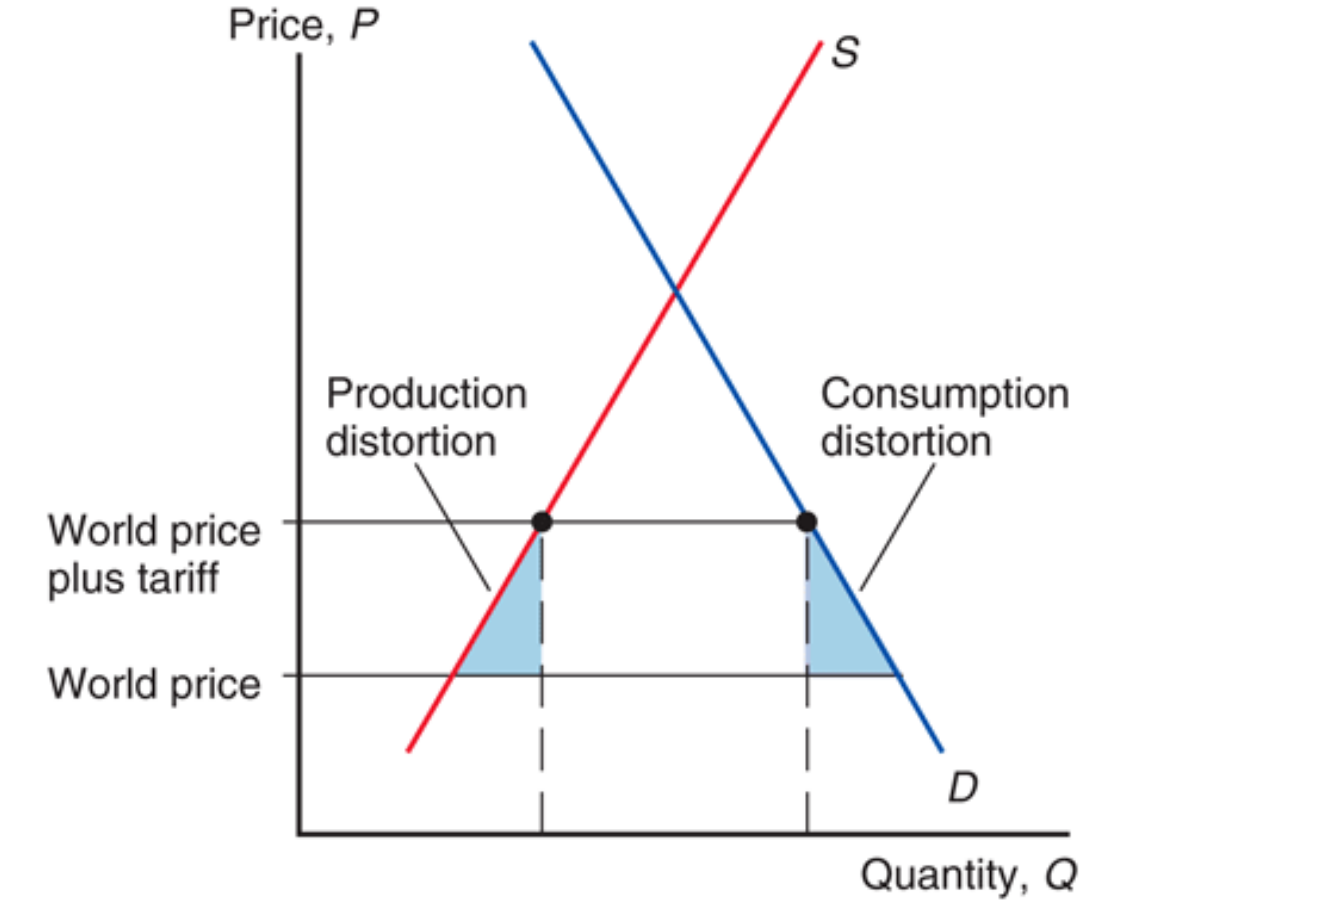
\includegraphics[scale=0.25]{tariff_distortion.png}

\end{frame}

\begin{frame}{Rent seeking distortions}

    \begin{itemize}
        \item Suppose we have import quotas
        \item How to allocate?
        \item Allocation system distorts production
        \begin{itemize}
            \item Example 1: India inport licenses based on capacity, build unneeded capacity
            \item Example 2: US Tuna import licenses first come first serve, warehouse in December, big rush on Jan. 1st
        \end{itemize}
        \item Side note: License Raj in India
    \end{itemize}

\end{frame}

\begin{frame}{Political Process and Corruption}

    \begin{itemize}
        \item Trade policy good in theory
        \item Politics is messy
        \begin{itemize}
            \item Even good intentioned policies likely to be captured by special interest groups
            \item Might cause even bigger distortions
            \item Here free trade is a second best 
        \end{itemize} 
        \item Similar argument to why one should follow unjust laws
    \end{itemize}

\end{frame}

\begin{frame}{Size of gains from free trade}
    \begin{itemize}
        \item Tariffs are already low, further gains small
    \end{itemize}
    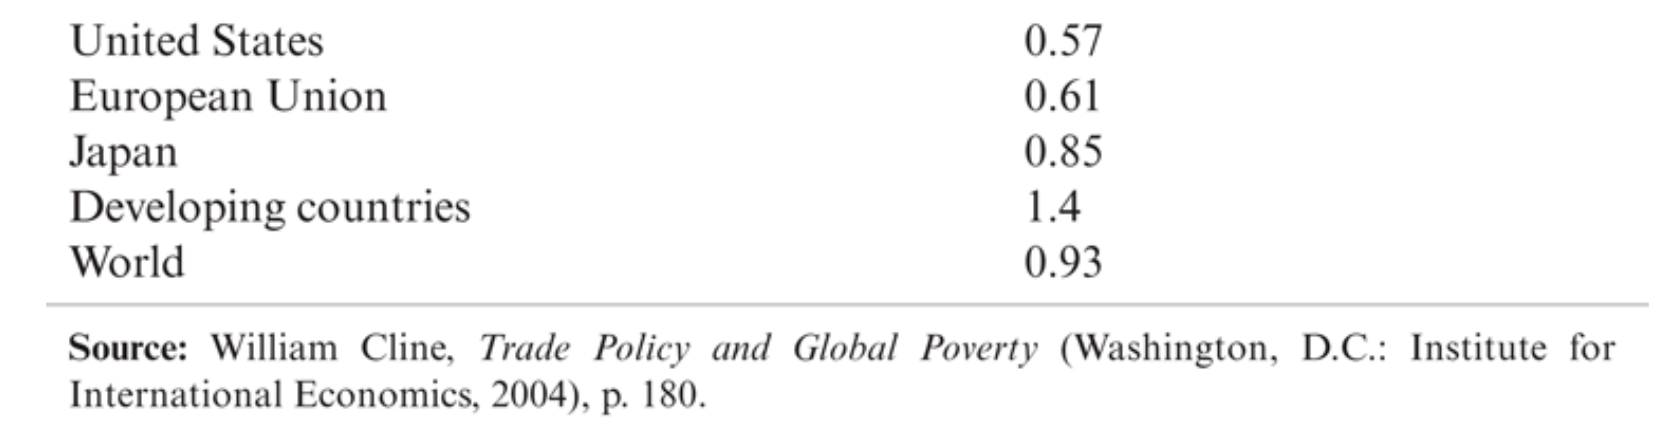
\includegraphics[scale=0.25]{trade_gains.png}
\end{frame}

\begin{frame}{Size of gains from trade}
    \begin{itemize}
        \item Research frontier: Gains from trade too small!
        \begin{itemize}
            \item We have arguments that countries gain from trade
            \item Recently theory models have been estimable
        \end{itemize}
        \item Important new paper: Gains from trade in most models are the same
        \begin{itemize}
            \item Arkolakis, Costinot, Rodriguez, American Economic Review, 2012
            \item United States going from autarchy to free trade welfare gains 0.7-1.4\% 
            \item Compare this to estimates of gains from migration\dots
        \end{itemize}
    \end{itemize}
\end{frame}

\begin{frame}{Gains from trade vs migration}
    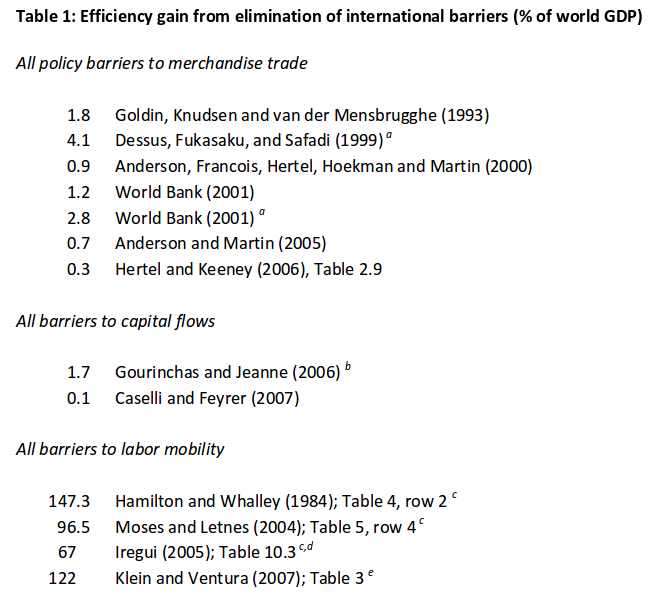
\includegraphics[scale=0.25]{gains_to_migration.png}

    {\tiny Source: Clemens, Michael, ``Economics and Emigration: Trillion Dollar Bills on the Sidewalk?'', Journal of Economic Perspectives, 2011}
\end{frame}

\begin{frame}{Pause}
    \begin{itemize}
        \item We have seen more arguments for free trade
        \begin{itemize}
            \item Classical gains from trade
            \item Trade policy causes rent seeking distortions
            \item Trade policy is often captured by special interests
        \end{itemize}
        \item Now we will focus on arguments against free trade
        \begin{itemize}
            \item The optimum tariff
            \item Domestic market failure and trade policy
        \end{itemize}
    \end{itemize}
\end{frame}

\begin{frame}{The optimum tariff}
    \begin{itemize}
        \item We saw that optimum tariff levels are always positive
        \item Same argument can be used to justify optimum export tax!
    \end{itemize}
    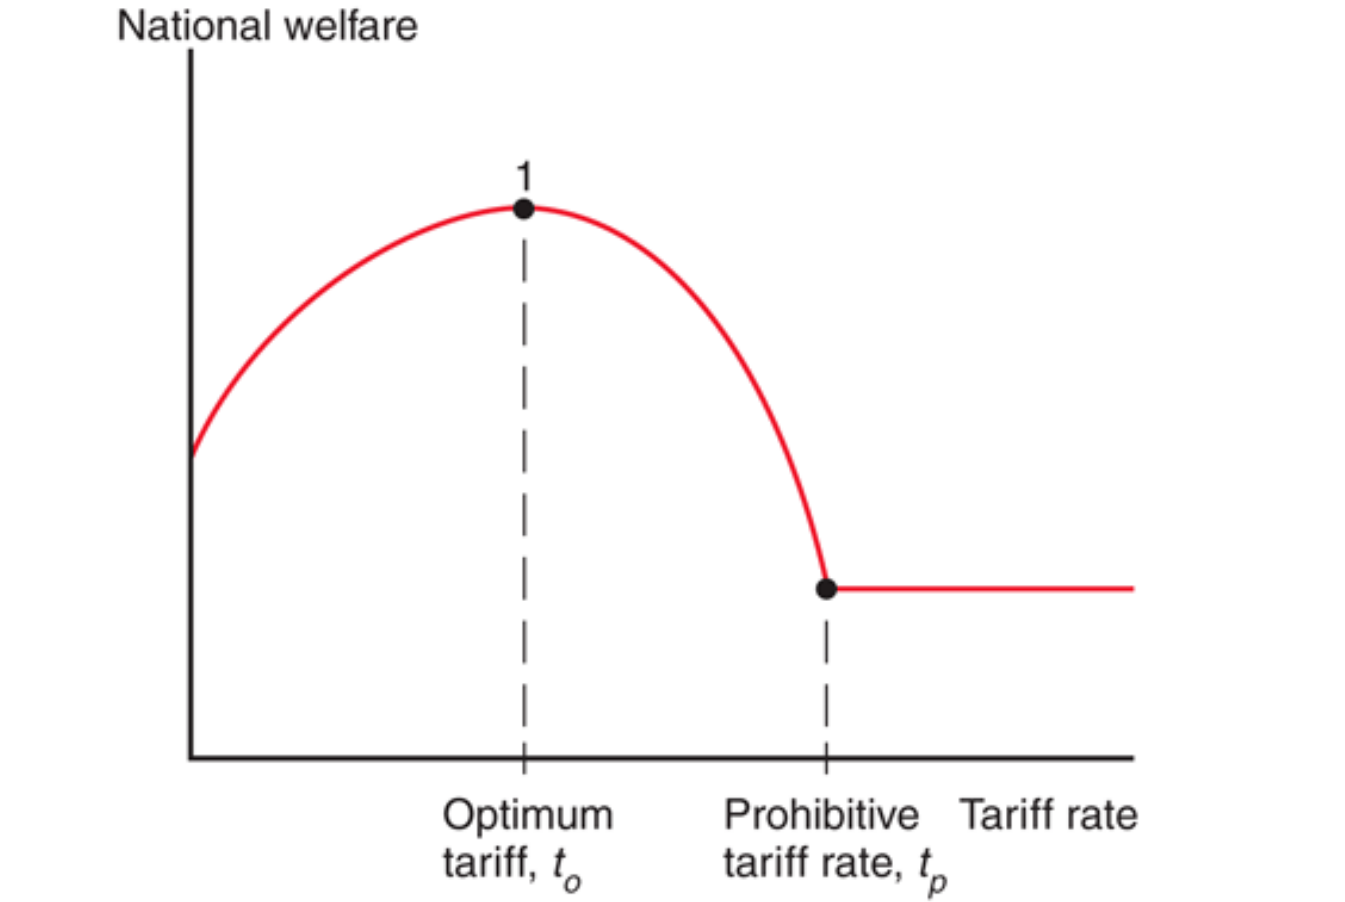
\includegraphics[scale=0.20]{optimum_tariff.png}
\end{frame}


\begin{frame}{The optimum tariff}
    \begin{itemize}
        \item Why do we rarely see export taxes?
        \item Why are tariff levels currently so low?
        \item Why don't large countries impose tariffs on small countries?
    \end{itemize}
\end{frame}

\begin{frame}{The market failure argument}
    \begin{itemize}
        \item Many US cities are congested with traffic 
        \begin{itemize}
            \item As Dane's you don't really understand this
            \item Chicago traffic, commute times
        \end{itemize}
        \item To reduce traffic problems
        \begin{itemize}
            \item Give firms a tax benefit to locating outside of city center
            \item OR raise toll on traffic going into the city
        \end{itemize}
        \item Economists typically support the toll, because it directly addresses the externality 
        \item Moving firms has all sorts of secondary effects
        \item But maybe the toll cannot be changed for some reason\dots
    \end{itemize}
\end{frame}

\begin{frame}{The theory of the second best}
    \begin{itemize}
        \item Markets are great, but plenty of market failures
        \begin{itemize}
            \item Traffic is one example of an externality
            \item Pollution is another
            \item Typically things worse in developing countries
        \end{itemize}
        \item The best policy is usually to tax the externality
        \item But if that isn't possible, maybe trade policy can help
        \begin{itemize}
            \item Suppose corruption makes it hard for new manufacturing firms to enter
            \item Too little manufacturing
            \item We could use trade policy to encourage entry into manufacturing
        \end{itemize}
        \item On the other hand
        \begin{itemize}
            \item It is hard to choose winners
            \item Effects of second-best costly and hard to predict
        \end{itemize}
    \end{itemize}
\end{frame}

\begin{frame}{Pause}
    \begin{itemize}
        \item We have seen more arguments for free trade
        \begin{itemize}
            \item Classical gains from trade
            \item Trade policy causes rent seeking distortions
            \item Trade policy is often captured by special interests
        \end{itemize}
        \item We have seen arguments against free trade
        \begin{itemize}
            \item The optimum tariff
            \item Domestic market failure and trade policy
        \end{itemize}
        \item Now we will talk about how trade policy is formed
    \end{itemize}
\end{frame}

\frame{
\frametitle{Political Models of Trade Policy}
Models related to trade policy:
\begin{enumerate}
\item Median voter theorem
\item Collective action
\end{enumerate}
}

\frame{
\frametitle{Median Voter Theorem}
Electoral competition can be modeled as:
\begin{itemize}
\item Two parties: Liberals ($L$) and the Greens ($G$)
\item Continuum of voters of size $N$
\item Line the voters up by their preferred tariff
\item A voter chooses the party closest to her preferred tariff
\item Parties take tariff positions to maximize support
\item Suppose that voters have a uniform distribution over preferred tariffs between $0$ and $T$
\end{itemize}
}

\frame{
\frametitle{Median Voter Theorem}
\begin{itemize}
\item Both parties choose the same, median voter supported trade policy 
\item What if there are three parties?
\item Median voter theorem predictions contrast with trade policy
\begin{itemize}
    \item Typically trade policy helps one industry a lot
    \item Typically trade policy hurts everyone else a little
\end{itemize}
\end{itemize}
}

\frame{
\frametitle{Collective Action}
\begin{itemize}
    \item Trade policy is a \emph{public good}
    \begin{itemize}
    \item That is, it cannot be excluded
    \end{itemize}
    \item Nearly everyone in EU hurt by agricultural export subsidies
    \item Suppose I write a letter to my representative
    \begin{itemize}
        \item The probability my letter is pivotal is small
        \item The benefit I get from removing subsidies is (relatively) small
        \item There is a small cost to sending a letter
        \item I won't do it
    \end{itemize}
    \item Suppose I am a EU farmer
    \begin{itemize}
        \item The probability my letter is pivotal is larger (smaller group of potential writers)
        \item The benefit I get from keeping subsidies is much larger
        \item There is a small cost to sending a letter 
        \item I do it
    \end{itemize}
    \item Result: All the letters from farmers
\end{itemize}
}

\frame{
    \frametitle{Punchline: Collective action}
    \begin{itemize}
        \item Policies with large aggregate loss but small individual loss are difficult to change
        \item Small groups with concentrated losses are more willing to pay effort fixed cost 
    \end{itemize}
}

\frame{
\frametitle{Real Politics}
\begin{itemize}
\item Politicians win elections partly because: 
    \begin{enumerate} 
        \item they advocate popular policies (median voter theorem)
        \item they have funds to run campaigns (collective action)
    \end{enumerate}
\item We expect trade policy in well-organized groups with concentrated gains 
\end{itemize}
}

\frame{
\frametitle{Which Industries are Protected?}
\begin{itemize}
\item Agriculture 
\begin{itemize}
    \item Small but politically vocal labor force in the US
    \item Japan has 1000\% tariff on rice imports!
\end{itemize}
\item Textiles (USA, about 14 \$ billion)
\begin{itemize}
    \item Declining in importance thanks to WTO
    \item Billions of dollars in US welfare loss due to protection:
\end{itemize}
\end{itemize}
    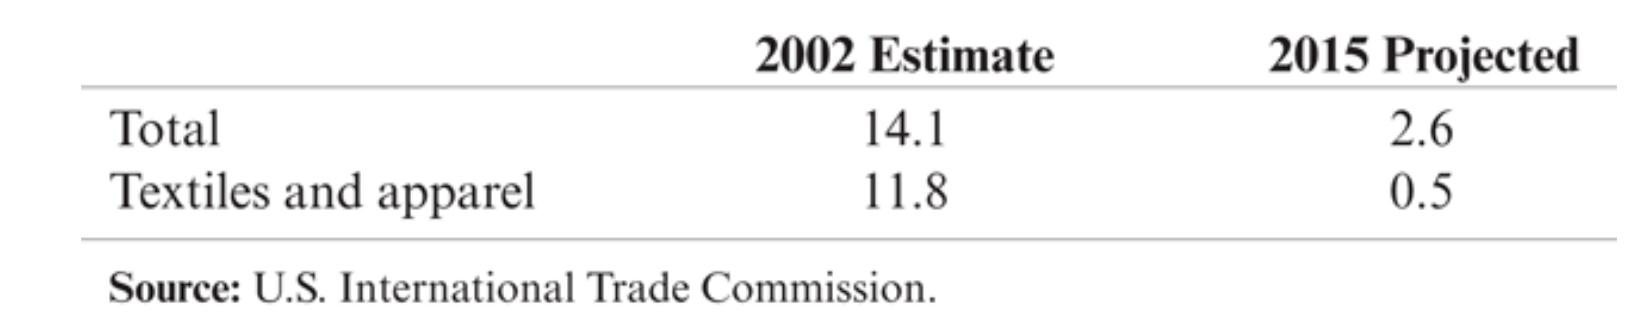
\includegraphics[scale=0.20]{textiles_welfare.png}
}

\begin{frame}{Pause}
    \begin{itemize}
        \item We have seen more arguments for free trade
        \begin{itemize}
            \item Classical gains from trade
            \item Trade policy causes rent seeking distortions
            \item Trade policy is often captured by special interests
        \end{itemize}
        \item We have seen arguments against free trade
        \begin{itemize}
            \item The optimum tariff
            \item Domestic market failure and trade policy
        \end{itemize}
        \item We have talk about how trade policy is formed
        \begin{itemize}
            \item Median voter
            \item Collective action
        \end{itemize}
        \item Next international negotiations
    \end{itemize}
\end{frame}

\frame{
\frametitle{International Negotiations}
\begin{itemize}
\item A US-centric history of trade milestones:
\begin{itemize}
    \item 1930: Smoot-Harley Act
    \item 1932: Bilateral negotiations
    \item 1947: Multilateral negotiations (GATT)
    \item 1995: WTO
\end{itemize}
\item US Tariff rates over the years
\end{itemize}
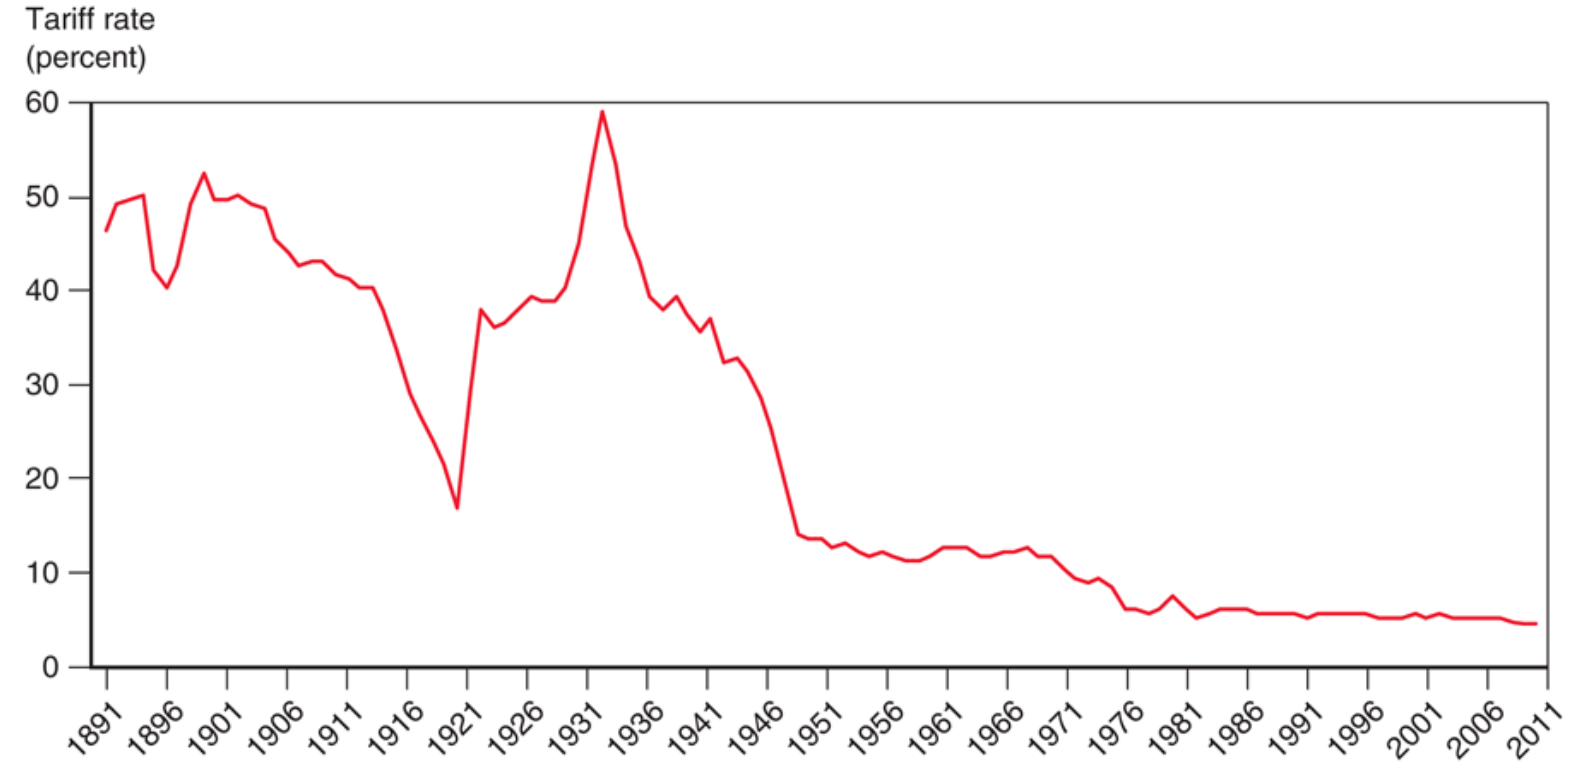
\includegraphics[scale=0.20]{tariff_rates_US.png}
}

\begin{frame}{Benefits of Trade Negotiations}
    \begin{itemize}
        \item Other countries will demand less protection from Home
        \item Nice way to counter special interests at Home
        \item Can also help avoid a trade war
    \end{itemize}
\end{frame}

\frame{
\frametitle{Trade War }
\begin{table}
\begin{tabular}{c c||c c|c c||}
 & & \multicolumn{4}{c||}{\textcolor{blue}{\textbf{European Union}}}\\\hline\hline
 & &   \multicolumn{2}{c|}{Free Trade} & \multicolumn{2}{c||}{Protection}\\\hline
\textcolor{red}{\textbf{US}}& Free trade &  &     &  &      \\\hline
&  &       &  & &      \\\hline\hline
\end{tabular}
\end{table}
}

\frame{
\frametitle{Trade War }
\begin{table}
\begin{tabular}{c c||c c|c c||}
 & & \multicolumn{4}{c||}{\textcolor{blue}{\textbf{European Union}}}\\\hline\hline
 & &   \multicolumn{2}{c|}{Free Trade} & \multicolumn{2}{c||}{Protection}\\\hline
\textcolor{red}{\textbf{US}}& Free trade &  & \textcolor{blue}{10B }     &  &   \textcolor{blue}{20B }   \\\hline
&  &       &  & &       \\\hline\hline
\end{tabular}
\end{table}
}

\frame{
\frametitle{Trade War }
\begin{table}
\begin{tabular}{c c||c c|c c||}
 & & \multicolumn{4}{c||}{\textcolor{blue}{\textbf{European Union}}}\\\hline\hline
 & &   \multicolumn{2}{c|}{Free Trade} & \multicolumn{2}{c||}{Protection}\\\hline
\textcolor{red}{\textbf{US}}& Free trade &  & \textcolor{blue}{10B }     &  &   \textcolor{blue}{$\underline{20B }$}   \\\hline
&  &       &  & &        \\\hline\hline
\end{tabular}
\end{table}
}

\frame{
\frametitle{Trade War }
\begin{table}
\begin{tabular}{c c||c c|c c||}
 & & \multicolumn{4}{c||}{\textcolor{blue}{\textbf{European Union}}}\\\hline\hline
 & &   \multicolumn{2}{c|}{Free Trade} & \multicolumn{2}{c||}{Protection}\\\hline
\textcolor{red}{\textbf{US}}& Free trade &  & \textcolor{blue}{10B }     &  &   \textcolor{blue}{$\underline{20B }$}   \\\hline
\textcolor{red}{\textbf{US}}&Protection  &       & \textcolor{blue}{-10B } & &  \textcolor{blue}{-5B }      \\\hline\hline
\end{tabular}
\end{table}
}

\frame{
\frametitle{Trade War }
\begin{table}
\begin{tabular}{c c||c c|c c||}
 & & \multicolumn{4}{c||}{\textcolor{blue}{\textbf{European Union}}}\\\hline\hline
 & &   \multicolumn{2}{c|}{Free Trade} & \multicolumn{2}{c||}{Protection}\\\hline
\textcolor{red}{\textbf{US}}& Free trade &  & \textcolor{blue}{10B }     &  &   \textcolor{blue}{$\underline{20B }$}   \\\hline
\textcolor{red}{\textbf{US}}&Protection  &       & \textcolor{blue}{-10B } & &  \textcolor{blue}{$\underline{-5B }$}      \\\hline\hline
\end{tabular}
\end{table}
}


\frame{
\frametitle{Trade War }
\begin{table}
\begin{tabular}{c c||c c|c c||}
 & & \multicolumn{4}{c||}{\textcolor{blue}{\textbf{European Union}}}\\\hline\hline
 & &   \multicolumn{2}{c|}{Free Trade} & \multicolumn{2}{c||}{\textcolor{blue}{Protection}}\\\hline
\textcolor{red}{\textbf{US}}& Free trade &  & \textcolor{blue}{10B }     &  &   \textcolor{blue}{$\underline{20B }$}   \\\hline
\textcolor{red}{\textbf{US}}&Protection  &       & \textcolor{blue}{-10B } & &  \textcolor{blue}{$\underline{-5B }$}      \\\hline\hline
\end{tabular}
\end{table}
}



\frame{
\frametitle{Trade War }
\begin{table}
\begin{tabular}{c c||c c|c c||}
 & & \multicolumn{4}{c||}{\textcolor{blue}{\textbf{European Union}}}\\\hline\hline
 & &   \multicolumn{2}{c|}{Free Trade} & \multicolumn{2}{c||}{\textcolor{blue}{Protection}}\\\hline
\textcolor{red}{\textbf{US}}& Free trade & \textcolor{red}{10B } & \textcolor{blue}{10B }     &  &   \textcolor{blue}{$\underline{20B }$}   \\\hline
\textcolor{red}{\textbf{US}}&Protection  &  \textcolor{red}{20B }     & \textcolor{blue}{-10B } & &  \textcolor{blue}{$\underline{-5B }$}      \\\hline\hline
\end{tabular}
\end{table}
}


\frame{
\frametitle{Trade War }
\begin{table}
\begin{tabular}{c c||c c|c c||}
 & & \multicolumn{4}{c||}{\textcolor{blue}{\textbf{European Union}}}\\\hline\hline
 & &   \multicolumn{2}{c|}{Free Trade} & \multicolumn{2}{c||}{\textcolor{blue}{Protection}}\\\hline
\textcolor{red}{\textbf{US}}& Free trade & \textcolor{red}{10B } & \textcolor{blue}{10B }     &  &   \textcolor{blue}{$\underline{20B }$}   \\\hline
\textcolor{red}{\textbf{US}}&Protection  &  $\textcolor{red}{\underline{20B }}$     & \textcolor{blue}{-10B } & &  \textcolor{blue}{$\underline{-5B }$}      \\\hline\hline
\end{tabular}
\end{table}
}


\frame{
\frametitle{Trade War }
\begin{table}
\begin{tabular}{c c||c c|c c||}
 & & \multicolumn{4}{c||}{\textcolor{blue}{\textbf{European Union}}}\\\hline\hline
 & &   \multicolumn{2}{c|}{Free Trade} & \multicolumn{2}{c||}{\textcolor{blue}{Protection}}\\\hline
\textcolor{red}{\textbf{US}}& Free trade & \textcolor{red}{10B } & \textcolor{blue}{10B }     &  \textcolor{red}{$\underline{-10B }$} &   \textcolor{blue}{$\underline{20B }$}   \\\hline
\textcolor{red}{\textbf{US}}&Protection  &  $\textcolor{red}{\underline{20B }}$     & \textcolor{blue}{-10B } & \textcolor{red}{$\underline{-5B }$}&  \textcolor{blue}{$\underline{-5B }$}      \\\hline\hline
\end{tabular}
\end{table}
}


\frame{
\frametitle{Trade War }
\begin{table}
\begin{tabular}{c c||c c|c c||}
 & & \multicolumn{4}{c||}{\textcolor{blue}{\textbf{European Union}}}\\\hline\hline
 & &   \multicolumn{2}{c|}{Free Trade} & \multicolumn{2}{c||}{\textcolor{blue}{Protection}}\\\hline
\textcolor{red}{\textbf{US}}& Free trade & \textcolor{red}{10B } & \textcolor{blue}{10B }     &  \textcolor{red}{$\underline{-10B }$} &   \textcolor{blue}{$\underline{20B }$}   \\\hline
\textcolor{red}{\textbf{US}}& \textcolor{red}{Protection}  &  $\textcolor{red}{\underline{20B }}$     & \textcolor{blue}{-10B } & \textcolor{red}{$\underline{-5B }$}&  \textcolor{blue}{$\underline{-5B }$}      \\\hline\hline
\end{tabular}
\end{table}
}


\frame{
\frametitle{"Ulysses and the Sirens" (1)}
\textit{But if you wish to listen, let the men tie you in the lugger, hand
and foot, back to the mast, lashed to the mast,
so you may hear those harpies' thrilling voices...}[Homer, Odyssey]
\begin{figure}
	\centering
		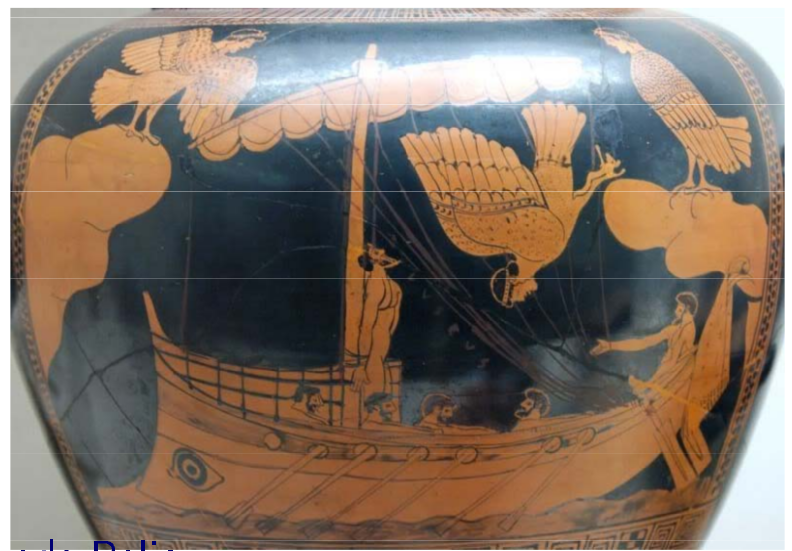
\includegraphics[width=0.75\textwidth]{ulysses.png}
\end{figure}
}

\frame{
\frametitle{"Ulysses and the Sirens" (2)}
If countries can establish a binding agreement to maintain free trade, both can avoid the temptation of protection and both can be made better off.
$\Rightarrow$ World Trade Organization (WTO)
\begin{enumerate}
\item Reduction of tariff rates 
\item Binding
\item Prevention of non-tariff barriers
\end{enumerate}
}

\begin{frame}{Trade War}
    \begin{itemize}
        \item Side note: Prisoner's dilemma not as bad if repeated
        \item How would does WTO affect the one-shot prisoner's dilemma?
    \end{itemize}
\end{frame}

\frame{
\frametitle{Trade War }
\begin{table}
\begin{tabular}{c c||c c|c c||}
 & & \multicolumn{4}{c||}{\textcolor{blue}{\textbf{European Union}}}\\\hline\hline
 & &   \multicolumn{2}{c|}{Free Trade} & \multicolumn{2}{c||}{\textcolor{blue}{Protection}}\\\hline
\textcolor{red}{\textbf{US}}& Free trade & \textcolor{red}{10B } & \textcolor{blue}{10B }     &  \textcolor{red}{$\underline{-10B }$} &   \textcolor{blue}{$\underline{5B }$}   \\\hline
\textcolor{red}{\textbf{US}}& \textcolor{red}{Protection}  &  $\textcolor{red}{\underline{5B }}$     & \textcolor{blue}{-10B } & \textcolor{red}{$\underline{-5B }$}&  \textcolor{blue}{$\underline{-5B }$}      \\\hline\hline
\end{tabular}
\end{table}
}

\begin{frame}{Pause}
    \begin{itemize}
        \item We have seen more arguments for free trade
        \begin{itemize}
            \item Classical gains from trade
            \item Trade policy causes rent seeking distortions
            \item Trade policy is often captured by special interests
        \end{itemize}
        \item We have seen arguments against free trade
        \begin{itemize}
            \item The optimum tariff
            \item Domestic market failure and trade policy
        \end{itemize}
        \item We have talk about how trade policy is formed
        \begin{itemize}
            \item Median voter
            \item Collective action
        \end{itemize}
        \item International negotiations and Trade Wars
        \item Last bit in Chapter 10: Preferential Trade Agreements
    \end{itemize}
\end{frame}

\frame{
\frametitle{Preferential Trade Agreement}
\begin{itemize}
    \item Only allowed under WTO if totally eliminate tariffs between partners
\end{itemize}
\begin{enumerate}
\item \textbf{free trade area:} an agreement that allows free trade among members, but each member can have its own trade policy towards non-member countries (e.g., NAFTA)
\item \textbf{custom unions:} an agreement that allows free trade among members and requires a common external trade policy towards non-member countries. (e.g., European Union)
\end{enumerate}
\begin{itemize}
    \item Surprisingly, entering a free trade area can make a country worse off!
    \item Some estimate that Mexico actually was made worse off by NAFTA
\end{itemize}
}



\frame{
\frametitle{Preferential Trade Agreement}
\begin{table}
\begin{tabular}{||l|c|c|c|c||}\hline \hline
 & \textbf{UK} & \textbf{F} & \textbf{US} & \textbf{UK import from}\\ \hline
$p$ & 8 & 6 & 4 & US \\ \hline
\multicolumn{5}{||c||}{$1^{st}$ case}\\ \hline
$p+t$ & 8 & 11 & 9 & -\\
CU with F & 8 & 6 & 9 & F (trade creation)\\ \hline
\multicolumn{5}{||c||}{$2^{nd}$ case}\\ \hline
$p+t^{2}$ & 8 & 9 & 7 & US\\
CU with F & 8 & 6 & 7 & F (trade diversion)\\ \hline
\end{tabular}
\end{table}
}

\frame{% how to print
\frametitle{}
\begin{center}
\textcolor{blue}{Chapter 11: Trade Policy in Developing Countries
}
\end{center}
}

\frame{% how to print
\frametitle{Import Substituting Industrialization}
Developing countries:
\begin{itemize}
\item Trade policy adopted by many developing countries before the 1980s (e.g., in Latin America 1950-60)
\item Encourage domestic industries (\textit{infant industries}) by limiting competing imports
\item End of colonialism
\begin{itemize}
    \item Common belief: poor countries exploited by rich countries through international financial markets and trade.
    \item Potential comparative advantage in manufacturing, need protection to start (External returns to scale)
\end{itemize}
\end{itemize}
but
\begin{enumerate}
\item Comparative advantages
\item In practice, corruption and monopoly
\item Market failures
\end{enumerate}
}

\frame{% how to print
\frametitle{In support of Infant Industries}
Market failures
\begin{enumerate}
\item Imperfect financial markets
    \begin{itemize}
        \item Good firms must reinvest profits to grow
        \item Protection increases producer surplus
    \end{itemize}
\item The problem of appropriability 
    \begin{itemize}
        \item Pioneering firms may pay sunk costs later entrants will not have to pay
        \item Protection is like a subsidy which may overcome one-time costs of entry
    \end{itemize}
\end{enumerate}
}

\frame{% how to print
\frametitle{History of Import Substitution}
\begin{enumerate}
\item Many countries in 1950's and 1960's subsidized domestic replacement of imports
    \begin{itemize}
        \item Justification from infant industry argument
        \item This policy also reduced exports (why?)
        \item Delinking the developing world
    \end{itemize}
\item Extreme protection
    \begin{itemize}
        \item India in early 1970's imported 3\% of its GDP (excluding oil)
        \item Effective tariff rates:
    \end{itemize}
		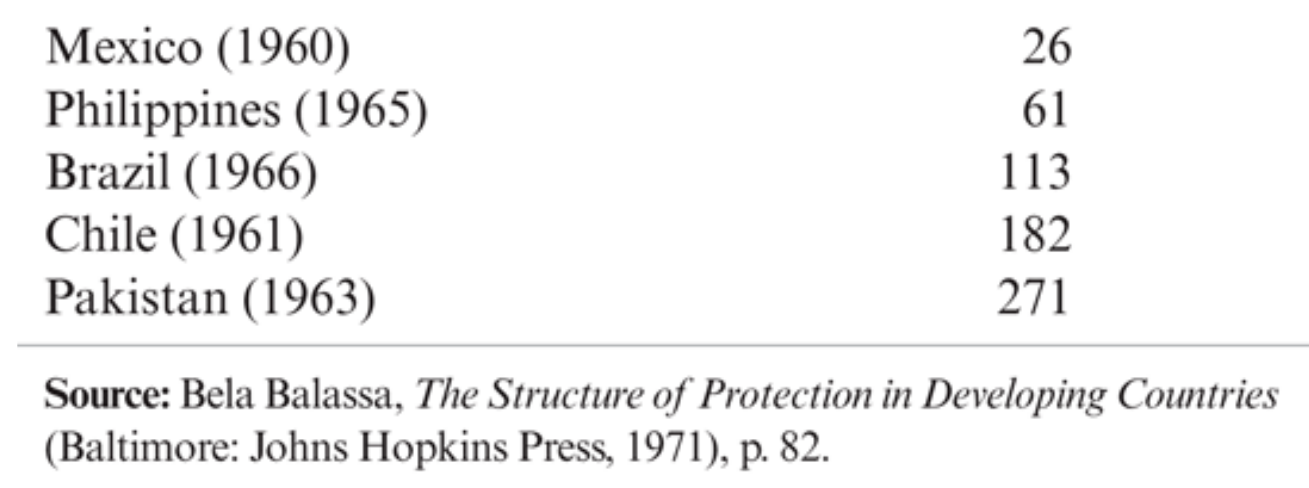
\includegraphics[width=0.75\textwidth]{effective_protection.png}
\end{enumerate}
}

\frame{% how to print
\frametitle{The End of Import Substitution}
\begin{itemize}
\item In the 1980's lost popularity
    \begin{itemize}
        \item One reason: emergence of export-growth led Asian tigers
        \item Also poor performance of import-substitution industries
    \end{itemize}
\item Reasons
    \begin{itemize}
        \item Production on too small a scale (external returns to scale)
        \item Protection badly distorted incentives through rent seeking: the raj
        \item Increased red-tape and regulation, increasing cost of starting a business
    \end{itemize}
\end{itemize}
}

\begin{frame}{The Asian Tigers}
		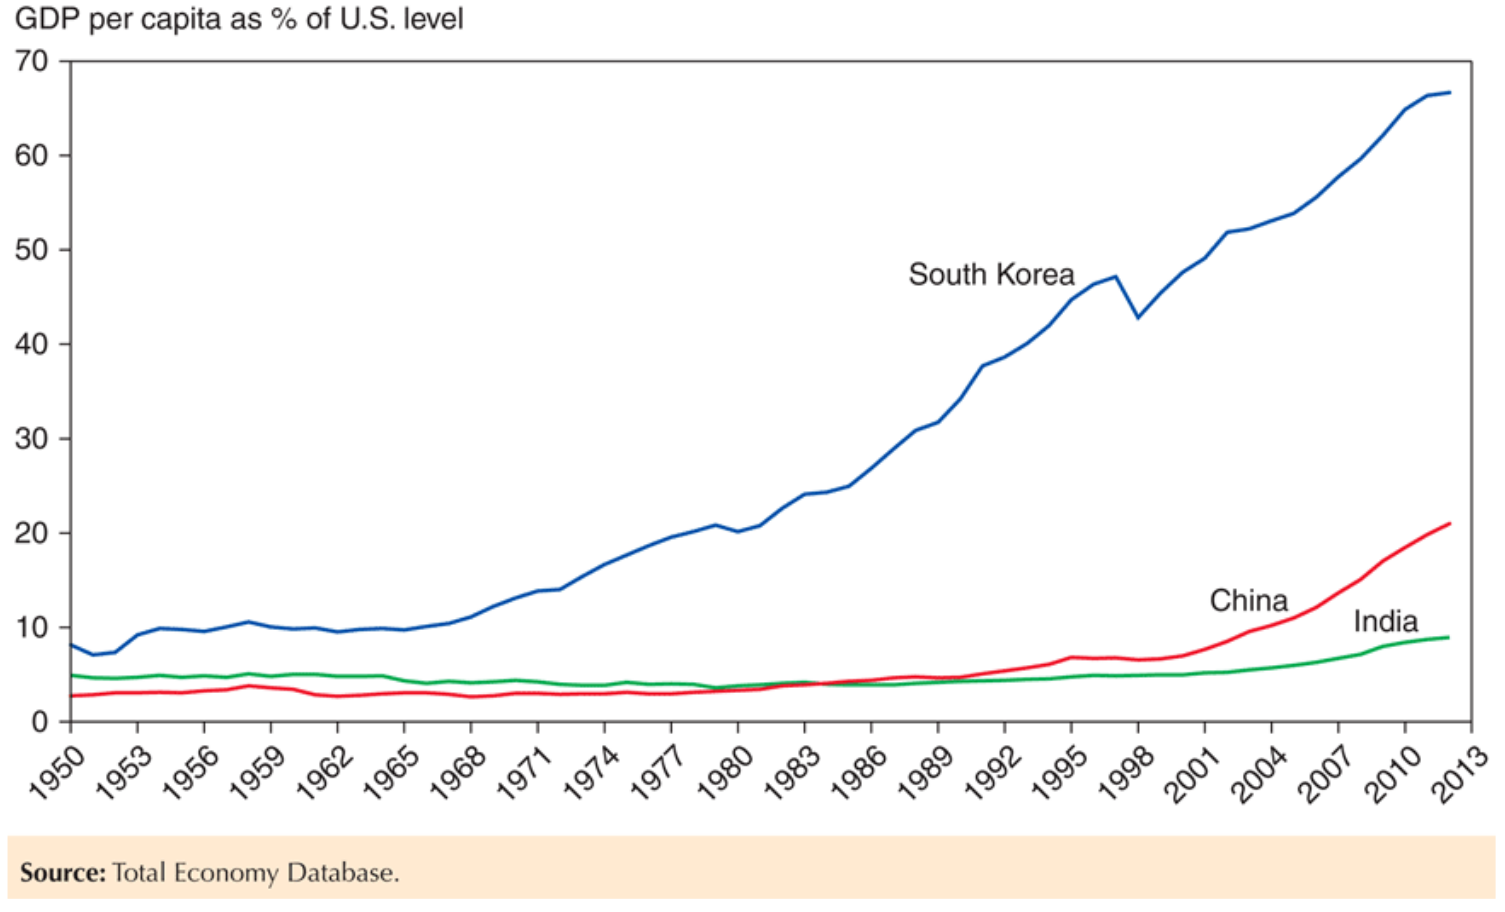
\includegraphics[scale=0.20]{tigers.png}
\end{frame}

\begin{frame}{The End of Import Substitution}
		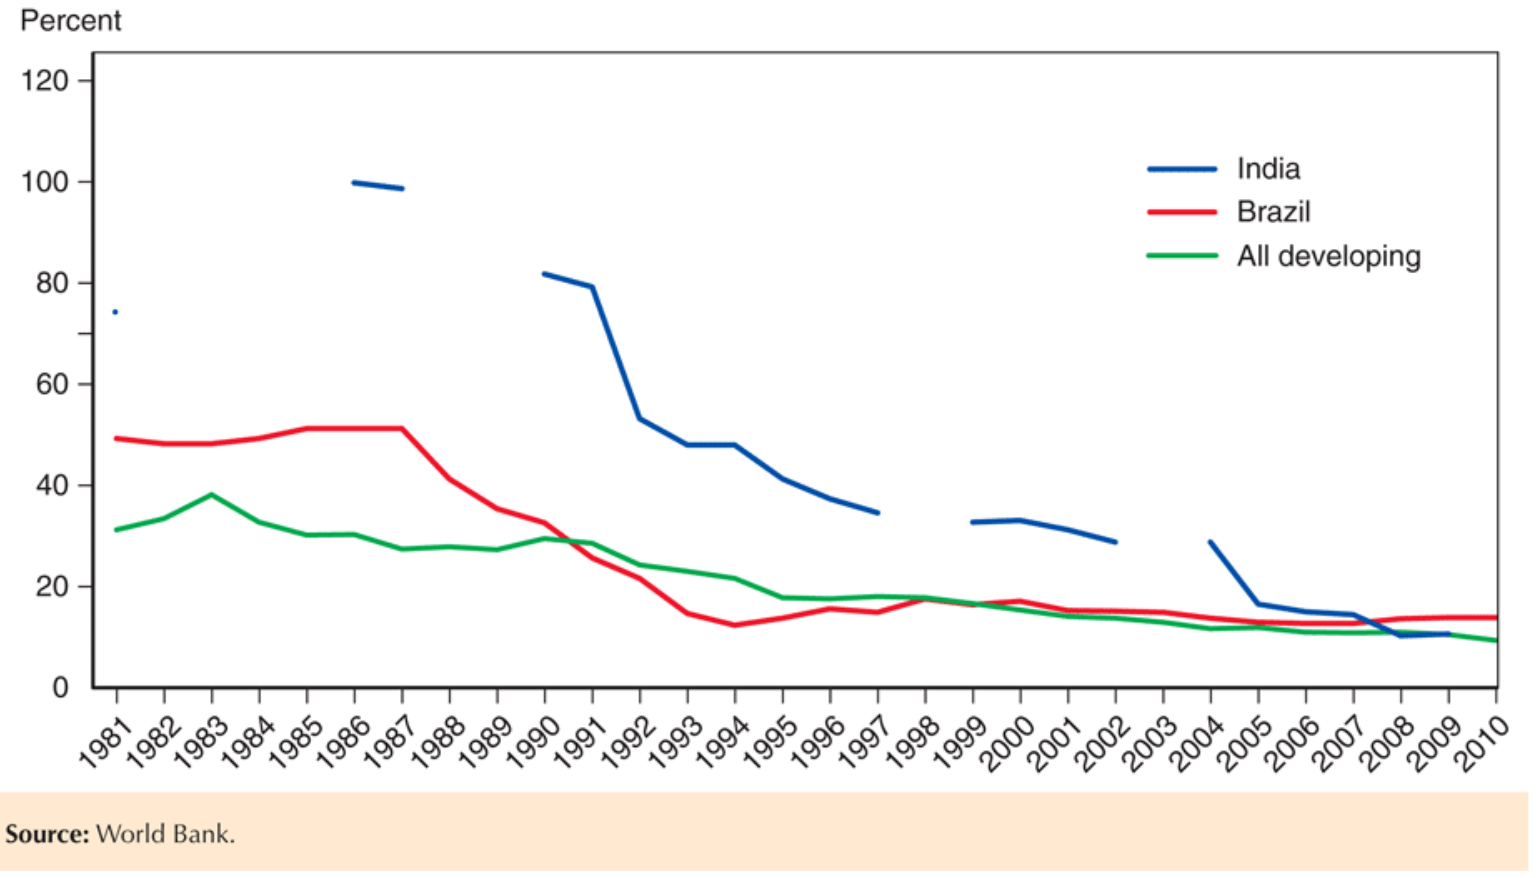
\includegraphics[scale=0.20]{tariff_decline.png}
\end{frame}

\begin{frame}{The End of Import Substitution}
		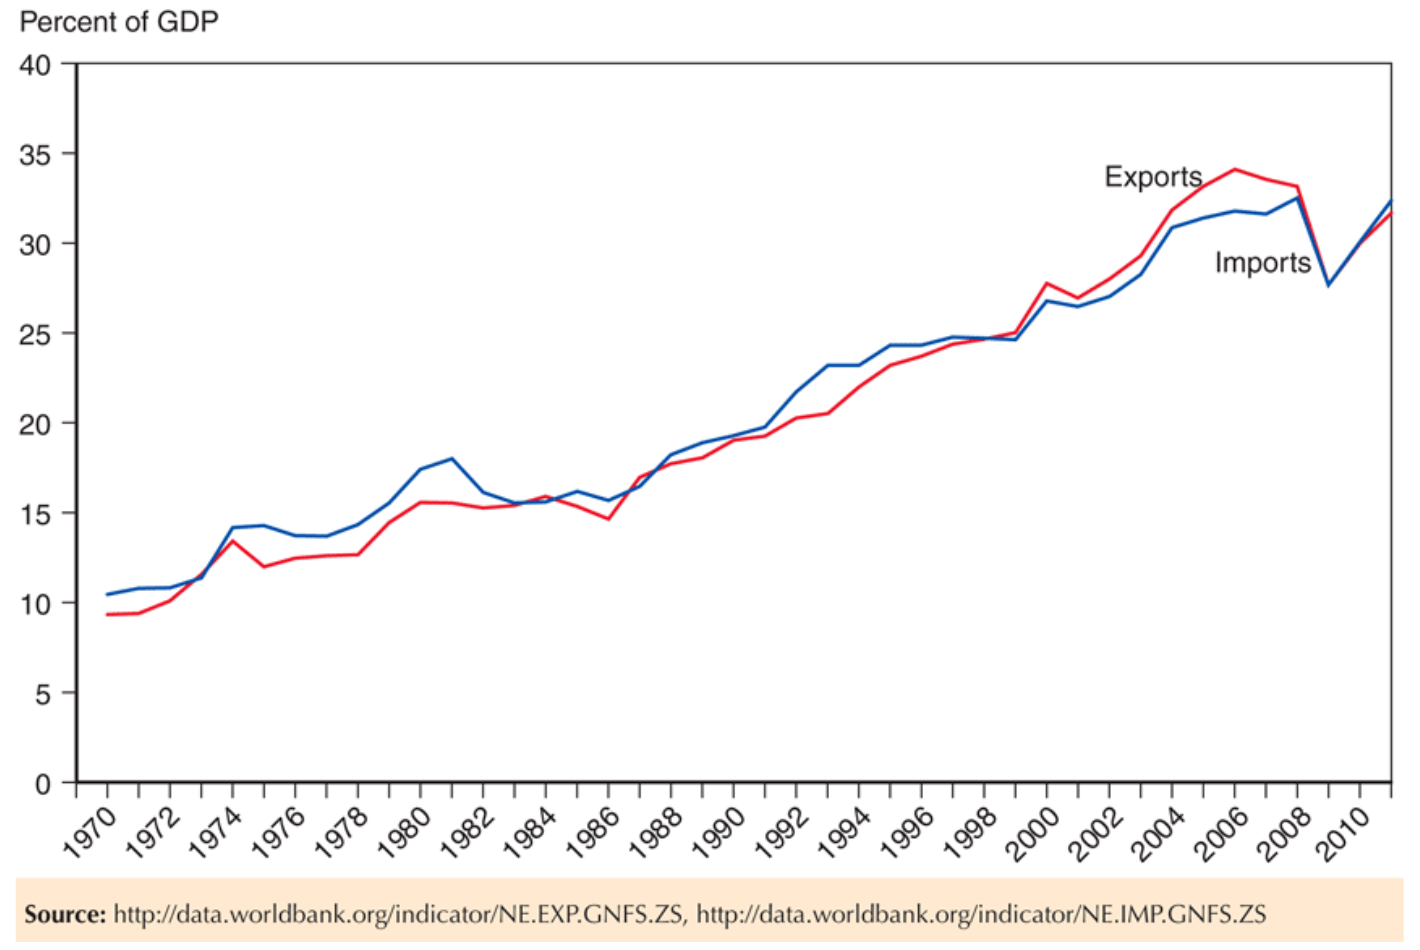
\includegraphics[scale=0.20]{develop_trade.png}
\end{frame}

\frame{% how to print
\frametitle{Trade Liberalization}
There is some evidence that low and middle income countries which had relatively free trade had higher average economic growth than those that followed import substituting industrialization (before mid-1980s).
}

\frame{
\frametitle{Export Oriented Industrialization}
\begin{itemize}
\item "high performance Asian economies" adopted trade policies that promoted exports in targeted industries
\item Although evidence suggests that these economies did have less restricted trade than other low and middle income countries, trade restrictions were still in effect. (causality or correlation ?)
\end{itemize}
}


\frame{
\frametitle{Average Rates of Protection, 1985 (percent)}
\begin{itemize}
    \item Still plenty of protection in the tigers
\end{itemize}
		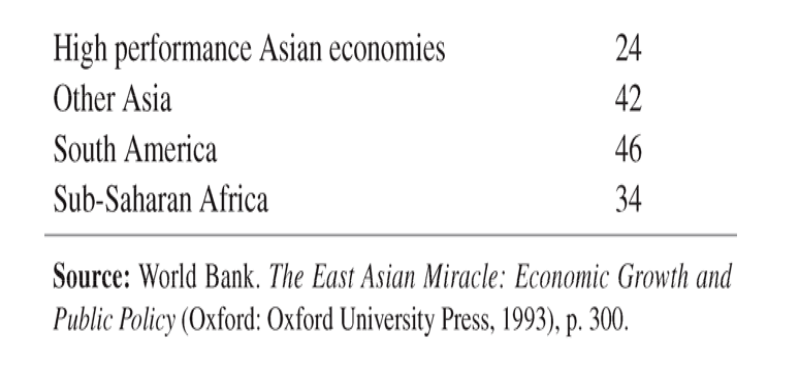
\includegraphics[scale=0.25]{plenty_of_protection.png}
}


\frame{% how to print
\frametitle{}
\begin{center}
\textcolor{blue}{Chapter 12: Controversies in Trade Policy
}
\end{center}
}

\frame{
\frametitle{Arguments for an Activist Trade Policy}
\begin{enumerate}
\item externalities
\item imperfect competition and monopoly rents 
\end{enumerate}
}

\frame{
\frametitle{Technology \& Externalities}
\begin{itemize}
    \item If good ideas can be copied, there is an externality to innovation
    \item Classic example: pharmeceuticals
    \item Might want to subsidize high marginal social benefit industries
    \item Problem: Government ability to target the right thing
\begin{itemize}
\item What is the next big innovation?
\end{itemize}
\end{itemize}
}

\frame{
\frametitle{Imperfect Competition and Strategic Trade Policy}
\begin{itemize}
\item Imperfectly competitive industries dominated by a few firms 
\item generate monopoly profits (excess returns).
\item Suppose a monopolistic firm sells a lot abroad
\item Government subsidies can shift excess profits to that firm.
\end{itemize}
}



\frame{
\frametitle{Profit Stealing (1)}
Suppose Boeing enters the market first and it decides to produce
\begin{table}
\begin{tabular}{c c||c c|c c||}
 & & \multicolumn{4}{c||}{\textcolor{blue}{\textbf{Airbus}}}\\\hline\hline
 & &   \multicolumn{2}{c|}{Produce} & \multicolumn{2}{c||}{\textcolor{blue}{Not Produce}}\\\hline
\textcolor{red}{\textbf{Boeing}}& \textcolor{red}{Produce} & \textcolor{red}{-5} & \textcolor{blue}{-5}     &  \textcolor{red}{$\underline{100}$} &   \textcolor{blue}{$\underline{0}$}   \\\hline
\textcolor{red}{\textbf{Boeing}}& Not Produce  &  $\textcolor{red}{{0}}$     & \textcolor{blue}{100} & \textcolor{red}{0}&  \textcolor{blue}{0}      \\\hline\hline
\end{tabular}
\end{table}
}

\frame{
\frametitle{Profit Stealing (2)}
\begin{itemize}
\item EU subsidize production by 25
\item Airbus will also produce independent of Boeing's decision
\item Boeing knows that and decides not to produce
\item $125 > 25 \Rightarrow$ social benefit
\end{itemize}
\begin{table}
\begin{tabular}{c c||c c|c c||}
 & & \multicolumn{4}{c||}{\textcolor{blue}{\textbf{Airbus}}}\\\hline\hline
 & &   \multicolumn{2}{c|}{\textcolor{blue}{Produce}} & \multicolumn{2}{c||}{Not Produce}\\\hline
\textcolor{red}{\textbf{Boeing}}& Produce & \textcolor{red}{-5} & \textcolor{blue}{20}     &  \textcolor{red}{100} &   \textcolor{blue}{0}   \\\hline
\textcolor{red}{\textbf{Boeing}}& \textcolor{red}{Not Produce}  &  \textcolor{red}{$\underline{0}$}     & \textcolor{blue}{$\underline{125}$} & \textcolor{red}{0}&  \textcolor{blue}{0}      \\\hline\hline
\end{tabular}
\end{table}
}

\frame{
\frametitle{Trade \& Environment}
\begin{itemize}
\item Environmental standards in low and middle income countries are lax.
\item Shifting maufacturing to developing countries pollutes
\end{itemize}
}



\frame{
\frametitle{The Environmental Kuznets Curve}
\begin{itemize}
    \item Empirical regularity: Pollution goes up as a country develops
    \item Side note: original Kuznets curve about inequality and development
    \begin{itemize}
        \item Developed in 1950s and 1960s when US was more equal
        \item Now looks pretty incorrect
    \end{itemize}
\end{itemize}
\begin{figure}
	\centering
		\includegraphics[scale=0.20]{kuznets.png}
	\label{fig:11}
\end{figure}
}

\frame{
\frametitle{The Rise of Chinese Pollution}
\begin{figure}
	\centering
		\includegraphics[scale=0.20]{chinese_pollution.png}
\end{figure}
}

\frame{
\frametitle{Pollution Havens}
\begin{itemize}
    \item Suppose EU laws want to clean up carbon pollution
    \begin{itemize}
        \item Makes it expensive for polluting firms to operate in EU
    \end{itemize}
    \item Why not move production to country with lax laws?
    \begin{itemize}
        \item Developing countries compete on laxness of environmental laws
        \item Pollution continues as before
    \end{itemize}
    \item Theoretically possible
    \item Empirically little evidence that this is happening
\end{itemize}
}
    
\frame{% how to print
\frametitle{Summary}
\begin{itemize}
    \item Chapter 10 : Politics and Trade Policy
    \begin{itemize}
        \item Some additional arguments for Free Trade
        \item Arguments Against Free Trade
        \begin{itemize}
            \item National Welfare reasons 
            \item Income Distribution and Trade Policy
        \end{itemize}
        \item International Negotiations
        \begin{itemize}
            \item Some theory
            \item A short history of International Trade Agreements 
            \item Preferential Trade Arrangements
        \end{itemize}
    \end{itemize}
    \item Chapter 11 : Developing Countries and Trade Policy
    \begin{itemize}
        \item Rise and Fall of Import Substitution 
        \item Export Oriented Industrialization
    \end{itemize}
    \item Chapter 12: Trade Policy Controversy
    \begin{itemize}
        \item More Arguments for an Activist Trade Policy
        \item Trade \& the Environment
    \end{itemize}
\end{itemize}
}

\begin{frame}{End of Trade Section}
\begin{itemize}
    \item Today was a catch-all for trade policy issues
    \item Next time start International Finance section!
\end{itemize}
\end{frame}

\end{document}
